\subsection{复活节}
\par
复活节(主复活日)是一个西方的重要节日,在每年春分月圆之后第一个星期日。基督徒认为,复活节象征着重生与希望,为纪念耶稣基督于公元30到33年之间被钉死在十字架之后第三天复活的日子。
\par
节日期间,人们按照传统习俗把鸡蛋煮熟后涂上红色,代表天鹅泣血,也表示生命女神降生后的快乐;大人孩子三五成群地聚在一处,用彩蛋作游戏;他们把彩蛋放在地上或土坡上滚,最后破裂者即为获胜,胜利者可以得到所有游戏者的彩蛋。该活动非常普通,即使是白宫,也要在复活节中组织这种游戏,不过这里是将彩蛋放在草坪上滚;人们相信,彩蛋在地上来回滚动可以使恶魔不断惊颤、倍受煎熬。这种风俗历史悠久,鸡蛋是复活节的象征,因为它预示着新生命的降临,相信新的生命一定会从中冲脱出世。
\par
在德国的巴伐利亚地区,每年的复活节居民们都要举行火炬赛跑,以庆祝耶稣的再生。而北莱茵上威斯特法伦州的吕克台复活节滚火轮更是远近闻名。六个巨型大木轮被火点燃滚下山谷,就像六个火球从天而降,漆黑的山谷被大火轮照得通明,它与五彩缤纷的焰火交相辉映,再次显示了火给人类带来了新生。作为德国唯一的少数民族索布族人则是用百骑大合唱的形式来庆祝耶稣的复活。一个个身穿黑色上衣、头戴黑色礼帽的索布族人,骑在用彩带、鲜花和白色贝壳装饰的骏马上,浩浩荡荡地行进在林间小路上。他们边走边用粗犷雄厚的嗓音高唱赞歌,场面十分壮观。
\begin{figure}[htb]
    \centering
    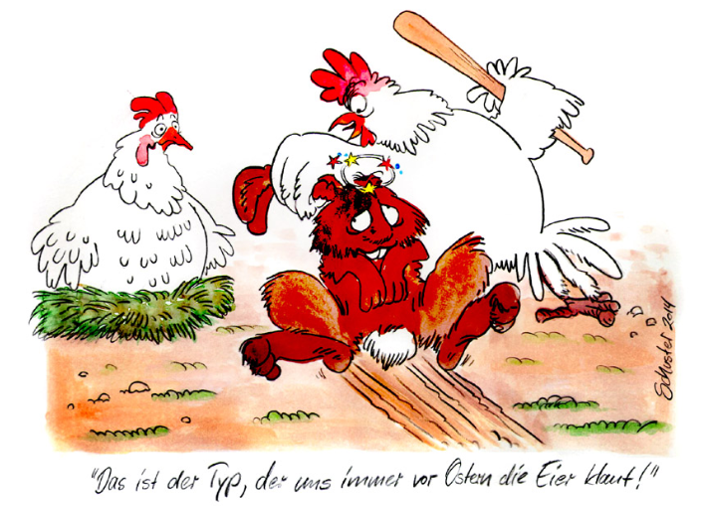
\includegraphics[width=0.5\linewidth]{fhjtz}
    \caption{复活节兔子}
    
\end{figure}

\subsection{圣灵降临节}
\par
圣灵降临节,被定于复活节后的第五十天,耶稣升天后第十天的主日,使徒们正聚集于耶路撒冷,圣灵突然从天而降,落在各人身上。于是众使徒大得力量,同别人广传福音,那天,约有三千人信了耶稣。之后又有五千人信仰基督,每天人数加增。因此,圣灵降临节就是初期基督教会诞生之日,十分重要。使徒们以后遂勇赴各地宣扬耶稣救人福音,而教会最后遂得以扩展至全世界。
\par
德国每年的圣灵降临节在圣诞前的第四个星期日正式开始,每个家庭都会在这期间买一个或自己扎一个枞树枝做的花环,上面插着的四支粗粗的蜡烛,并带有雪人、天使、圣诞老人或彩球等装饰。在节前的第四个礼拜天,也就是第一个圣灵降临节星期日,所有的家庭会点燃那四根蜡烛中的一支,在第二个星期日点燃第二支,当四支蜡烛都点燃了的时候,圣诞节也就近在眼前了。在这期间,很多家庭都会烤制圣诞小饼干,有巧克力的、有椰奶的、有水果夹心的、有奶油杏仁的,各式各样,无法尽数